% !TeX root = ./subthemeReport.tex

\documentclass[12pt,a4paper,titlepage]{jreport}
\usepackage{indentfirst}
\usepackage[dvipdfmx,hiresbb]{graphicx}
\usepackage{comment}
\usepackage{here}
\usepackage{enumerate}



%\input{link.bib}
%各種パッケージ
%\usepackage{...}


\title{副テーマ研究報告書 \\ 隔離ネットワークにおける通信制御の調査}


\date{\today}\author{\\ \\ \\1910225 嶂南 秀敏\\ \\
\\ \vspace{1mm}副テーマ指導教員 知念 賢一 特任准教授}


\begin{document}

\maketitle



\begin{abstract}
    
    \if0
     近代の情報インフラとしてのコンピュータシステムは経済活動や社会生活にとって欠くことのできない存在として、
    水道やガス電気と同じような安定性、信頼性が求められている。
    情報の保存・伝達方法の変化により、データの流通量が爆発的に拡大し、データの量・質・種類に多様化が生じた。
    これらのデータは政治、ビジネス、科学技術、災害対策など、様々な社会活動に利用され、我々の生活に大きな影響を与える事となった。
    インターネットの普及に伴い、安全なインターネットの利用に向けた課題が取り沙汰されるようになり、
    \fi
    現在、ユーザの遠隔サーバへの利用を容易にするアプリケーションは多く存在する。
    その一方で、サーバーへの通信接続をシステム管理者が容易に制御管理するためのアプリケーションは少ない。
    そのような通信制御のアプリケーションなしでは、システム管理者はユーザーの接続ごとに手動でコマンドを実行し
    管理しなければならず、サーバーを利用するユーザーが多くなるに従いシステム管理者への負担が多くなってしまう。
    \\
    \ そこで、本研究ではサーバーへの通信制御に有効なアプリケーションを調査することを目的とし、三台のサーバーと
    一台のL2スイッチを用いて隔離ネットワークを構成し、ゲートウェイサーバーに個人のソースコード投稿サイトに公開されている
    通信制御のアプリケーションを試用することで、通信制御の容易さ、通信の可視化度合い、セキュリティ、三点について検討を行う。
    
\end{abstract}

\tableofcontents
\clearpage
\chapter{はじめに}

\section{研究背景}
クラウドサーバーサービスの普及により、一般ユーザーが遠隔サーバーにアクセスし、その資源を利用する機会が増えてきた。
Googleのクラウドサービス(GCP)、Amazonのクラウドサービス(AWS)、Microsoftのクラウドサービス(Azure)などのように
ユーザーの目的に合わせて、遠隔サーバーの利用を容易にするアプリケーションが多く存在する。
しかし、一方でサーバーへの通信接続をシステム管理者が容易に制御管理するためのアプリケーションは少ない。
そのような通信制御のアプリケーションなしでは、システム管理者はユーザーの接続ごとに手動でコマンドを実行しなければならず、サーバー
を利用するユーザーが多くなるに従いシステム管理者への負担が多くなってしまう。\par
令和2年現在新型コロナウィルス感染症の世界的大流行により在宅勤務(テレワーク)が推奨され、
自宅から社内サーバーへのアクセスを余儀なくされている。そして、同年7月下旬に政府が在宅勤務7割を企業に要請した\cite{covid_nikkei}
ことにより、今後ますますテレワークの人口が増大していきそれに伴い、大規模なリモートアクセスにおけるセキュリティがより重要になり、
社内のシステム管理者の負担がますます増加していくことが予想できる。\par 






%ここで現在の課題や実社会でのネットワーク構成やアクセス図、セキュリティの問題点などを記す。


%社内システム管理者はテレワークによる社外ネットワークからの大規模アクセスのためにも、自社のネットワーク構成を
%見直す必要があるかもしれない。
%\\\\
%また、アプリケーションの適応先で小規模、大規模専用のものと分類し、その中で使われている技術についても解説を行う。
%\\\\

\section{研究目的}
%本研究では、図1のような隔離ネットワークを構成し、そこにソースコード投稿サイトに公開されている通信制御アプリケーションを試用し、
%その中で小規模と大規模アプリケーションいうように分類し検討を行う。


総務省テレワークセキュリティガイドラインには、テレワークの利用方法が6パターンに分類されており、それとともに
対策すべき観点もまとめられている。\cite{telework_guideline}それを以下の表\ref{telework_table}に示す。
下表\ref{telework_table}によると6パターンのうち1、2、6の3パターンが外部から社内サーバにアクセスを必要とする「オンプレミス型」のもので、
3、4、5の3パターンはインターネット上のクラウドサービスを利用している「クラウドサービス型」である。

\begin{table}[h]
    \centering
    \includegraphics*[width=0.9\textwidth,page=1]{graphs/telework_list.pdf}
    \caption{テレワークの6種類のパターン}
    \label{telework_table}
\end{table}

それぞれのパターンの細かな違いは、テレワーク利用端末にデータを保存できるかなどであり、
オンプレミス型もクラウドサービス型どちらもインターネットを介して、サーバにアクセスしている。
\par 本研究では、社内ネットワークを想定した、隔離ネットワークを構成し、そこにソースコード投稿サイトに公開されている
通信制御アプリケーションを試用することで、
その中で小規模と大規模アプリケーションで分類し検討を行うとともに、そこで使用されている遠隔アクセス技術、認証技術の解説も行う。

本研究でまとめることで、ブラックボックス的にリモートアクセスを行うのではなく、
どのような技術や仕組みを用いて実現しているか、高いセキュリティの実現のためにどのようなプロトコルを用いているかを、
リモートアクセス利用者の理解を深めることを目的とする。
それと同時にシステム管理者が通信接続の制御をすることを容易にするためのアプリケーションを調査する。
%ソースコード投稿サイトに公開されているアプリケーションの中には、商用としている一部を
%オープンソースとして公開しているものも存在する、



\begin{figure}[h]
    \centering
    \includegraphics*[width=0.8\textwidth,page=14]{graphs/network_archtecture.pdf}
    \caption{ クラウドサービス型}
    \label{cloud_graph}
\end{figure}


\begin{figure}[h]
    \centering
    \includegraphics*[width=0.8\textwidth,page=15]{graphs/network_archtecture.pdf}
    \caption{オンプレミス型}
    \label{onpremise_graph}
\end{figure}




\chapter{遠隔アクセス技術}
本章では遠隔サーバーに接続し操作するための技術やソフトウェアの解説を行う。

\section{暗号化技術}
暗号化技術は、情報の保護やコンピュータセキュリティに欠かせない技術である。
通信内容の保護のために、一般的に次に示す二種類の暗号化技術を使用して、認証及び暗号化通信を行っている。
\begin{itemize}
    \item 共通鍵暗号方式
    \item 公開鍵暗号方式
\end{itemize}
それぞれの暗号方式は様々なアルゴリズムによって実現されるが、元となる「平文」データを「鍵」を使って「暗号文」に変換している。
また、「暗号文」は「鍵」を使用して、「平文」に復号できる。

\subsection{共通鍵暗号方式}
AとBで共通の鍵を使用して、暗号化と復号化を行う。
そのため、暗号化通信をする前にこの共通鍵を事前に秘密に共有する必要がある。
共通鍵暗号方式の暗号化を下図\ref{shared_key}に示す。

共通鍵暗号方式は、後述の公開鍵暗号方式に比べて、演算の処理量が少ないとういう利点ある。
そのため、SSHプロトコルでは、通信内容の
暗号化にはこの共通鍵暗号方式を採用している。

\begin{figure}[h]
    \centering
    \includegraphics[width=0.9\textwidth, page=8]{graphs/network_archtecture.pdf}
    \caption{共通鍵暗号方式での暗号化}
    \label{shared_key}
\end{figure}

代表的な暗号化アルゴリズムに「AES」が存在する。
\subsection{公開鍵暗号方式}
公開鍵暗号方式は、二種類の鍵である公開鍵と秘密鍵をペアで使用する。この公開鍵と秘密鍵には次に示す性質があり、公開鍵暗号方式はこれら
の性質を利用して暗号化や署名を実現している。
\begin{itemize}
    \item 公開鍵で暗号化した平文は、秘密鍵で復号できる
    \item 公開鍵で暗号化した平文は、公開鍵では復号できない
    \item 秘密鍵で暗号化したデータは、公開鍵で復号できる
    \item 公開鍵から秘密鍵を生成できない。
\end{itemize}

公開鍵暗号方式での暗号化について下図\ref{public_key}に示す。この図では、鍵ペアを作成したBが、公開鍵をAに公開してる。Aは、Bの公開鍵を使用して
平文を暗号化して、Bへ送付する。送付された暗号文は、B自身の秘密鍵でのみ復号できる。

\begin{figure}[h]
    \centering
    \includegraphics[width=0.9\textwidth, page=9]{graphs/network_archtecture.pdf}
    \caption{公開鍵暗号方式での暗号化}
    \label{public_key}
\end{figure}

代表的な暗号化アルゴリズムに「RSA暗号」「Diffi-Hellman鍵共有」等がある。



\section{トンネリング(Tunneling)}\label{Tunnel}
ここでは、トンネリングの概要と\ref{aboutVPN}節に関係するVPNトンネリングプロトコルの説明を行う。

\subsubsection*{トンネリングとは}

トンネリングとは、「パケットやフレームを他のパケットやフレームの中にカプセル化すること」である。
これにより、プライベートアドレスの隠蔽や、カプセル化後に暗号化をすることでデータの保護を行うことができる。
後に説明するVPNにおいてもトンネリング技術は必要不可欠なものとなっている。
%トンネリングはVPNにおいてとても大切な役割を持つが、
ただし、
「トンネリング=VPN」であるわけではないというのは重要な点である。
%トンネルはVPNであるというわけではなく、VPNはトンネルであるというわけではないというのはとても重要な点である。

\par トンネリングの機能を以下に示す。
\begin{itemize}
    \item データ転送の容易化 \mbox{}\\
    トンネリングには、パケットまたはフレーム全体を直接特定の場所に転送する、「宛先を切り替える」
    機能を持つ。これにより、それらが宛先ネットワークに到着するとそのネットワークを管理している組織のセキュリティや
    ネットワークポリシーによる制御を受けることができる。
    \item 組み込みセキュリティ機能\mbox{}\\
    トンネリングプロトコルの中では、追加セキュリティ(暗号化、認証など)がプロトコルに組み込まれているもの
    がある。そのようなプロトコル(プロトコル群)の代表例として「IPSec」、「L2TP」や「PPTP」がある。
\end{itemize}


\subsection{IPSec}
IPSec(IP Security Architecture)は、IPパケットのデータの完全性(Integrity)と機密性(Confidentiality)を
保証する機能を
持っているプロトコル(プロトコルの集合)であり、ネットワーク層で動作しIPプロトコルでしか使用できない。
これらの機能を提供するための方法として、IPSecは以下の3つの要素を持ち、「AH」、「ESP」、「IKE」などの
プロトコルから構成されている。
\begin{itemize}
    \item 認証(ユーザレベルでなく、パケットレベルの)\mbox{}\\
    データの送信者が間違いなく本人であること、及び送信されたデータが受信されたデータと同一であることを
    検証する動作である。\par
    実現のためのプロトコル: AH、ESP
    \item 暗号化\mbox{}\\
    適切な鍵を持たない人にはデータを読み取ることができないようにする動作である。\par
    実現のためのプロトコル: ESP
    \item 鍵管理\mbox{}\\
    送信者と受信者の間でセキュリティ「鍵」の値を一致させたり、取り決めさせたりする動作である。\par
    実現のためのプロトコル: IKE
\end{itemize}
%IPSecにおけるパケットレベルの認証にはIPSecのAuthentication Header (認証ヘッダー) が使用される。

%\subsubsection*{IPSecを構成する2つのプロトコルと鍵交換のプロトコル}
\subsubsection{IPSecを構成するプロトコル}

\begin{itemize}
    \item AH(Authentication Header)\mbox{}\par
    パケットが改ざんされていないかどうか認証を行うが、パケットの暗号化はできない。\\RFC2402\cite{RFC2402}で定義されている

    \item ESP(Encapsulated Security Payload)\mbox{}\\
    パケットが改ざんされていないかどうか認証を行い、
    パケットのペイロード部の暗号化(DES or 3DES or AES)を行う。\\RFC2406\cite{RFC2406}で定義されている。 
    \item IKE(Inernet Key Exchange)\mbox{}\\
    秘密鍵情報の交換を安全に行う。(Difiie-Hellman鍵共有などを用いる)
    \\RFC2409\cite{RFC2409}で定義されている。
\end{itemize}

%\subsubsection*{IPSecの動作}
%IPSecは送信側と受信側というように、常に二組のユーザが関わりを持つ。IPSecの用語では
%このような関係をSA(Security Association)と呼ぶ。
IPSecでは、事前に通信を行うホスト同士が認証・暗号化のアルゴリズムや暗号鍵を共有するコネクションを形成
する必要がある。この関係をSA(Security Association)という。\par
IPSecに対応したホストやファイアウォールではデータベース内に複数のSAを保有することができ、あるIPSec
のパケットがどのSAに対応しているかは、IPSecのヘッダ中に含まれるSPI(Security Parameters Index)というポインタに指定される。
\par 
\subsubsection*{通信モード}
IPSecは通信モードが2つあり、「トンネルモード」と「トランスポートモード」である。
ここでは2つのモードを簡単に説明する。

まず、「トンネルモード」では、
    それぞれ別のネットワークとして構成されているネットワークで発生する通信パケットを、ゲートウェイでカプセル化して
    転送する。つまり、元のIPパケットをゲートウェイで「外側」のIPパケットの内部にカプセル化し、
    元のパケットをペイロード(正味のデータ部分)としてまったく新しいパケットを作成し転送している。
    その後ゲートウェイのIPに従って経路制御され、通信相手のゲートウェイでカプセル化されたパケットが取り出され、
    宛先となっているネットワークに配送される。

次に「トランスポートモード」は、
端末間でのIPSec通信を実現するために、転送する前に元のパケットのペイロードだけを暗号化する。
このとき、IPヘッダは暗号化されず、そのまま経路制御のために利用される。


\subsection{PPTP}
PPTP(Point-to-Point Tunneling Protocol)\cite{RFC2637}はデータリンク層で動作するトンネリングプロトコルの一つである。
リモートクライアントからプライベートな企業のサーバーにデータを安全に伝送することをようにするための手段として
設計された。サーバ/クライアントモデルで、データリンク層でカプセル化を行う。最も古いVPNプロトコルの一つであるが
設定が最も容易で計算速度が速いため、古く遅いデバイスで使用される。
深刻なセキュリティ上の脆弱性が存在するため、2020年現在使用することは勧められていない。
\subsubsection*{PPTPの通信手順}
以下にPPTPの通信手順を簡単に説明する。
\begin{enumerate}
    \item 制御用コネクションの確立(PPTPトンネルのための準備)\mbox{}\\
    トンネルの構築、維持、切断処理のための制御情報をやり取りするために、トンネル以外に制御用
    情報の交換のためのコネクションを確立している。制御コネクションにはTCPを利用している。
    \item PPPセッションを利用してPPTPトンネルを構築\mbox{}\\
    ここでは、PPP(Point-to-Point Protocol)が本来持っている仕組みを利用して、PPTPトンネルを構築するための
    認証及び暗号化の方法を選んで、実際に認証と鍵交換を行う。
\end{enumerate}

\subsection{L2TP}
L2TP(Layer 2 Tunneling Protocol)\cite{RFC2661}はL2F(Layer 2 Forwarding Protocol)とPPTPのアップグレードとして設計された。
VPNに利用することができるが、L2TPそのものは暗号化の仕組みを持っていないため、IPSecの暗号化機能と組み合わせて
VPNの暗号化通信を実現している。
L2TPはIPSecとは異なり、実装次第でトンネルするネットワークが必ずIPネットワークである必要がない。
そして、重要な点としてL2TPではカプセル化されたデータはUDPのデータとして(L2TPのメッセージとして)IPネットワーク上を配送
される。
\subsubsection*{L2TPの通信手順}
L2TPでは以下のような手順で通信経路の確立を行う。
\begin{enumerate}
    \item 初めに制御コネクションを確立してトンネルを構築する。
    \item その後同じトンネルを使ってユーザセッションを確立する。
    \item 最後にPPPによるリンクを確立する。
\end{enumerate}


\section{Telnet}
Telnetは、ネットワークに接続された機器を遠隔操作するために使用するアプリケーション層の技術である。
サーバ・クライアント方式で提供され、Telnetサーバが操作される側、クライアントが操作する側で動作する。
Telnetを使うことでオフィスのデスクにいながら、マシンルームにあるサーバ、ルータ等の機器をパソコン上で操作できる。
PCにはtelnetクライアント、ルータなどの機器にはtelnetサーバーのサービスが有効であることが前提である。
基本的にはポート番号23を使用する。


\subsection{Telnetの仕組み、使用法}
Telnetの接続までの流れは以下の図\ref{telnet_flow}のようになっている。
PCからのTelnetはコマンドプロンプトやTerminalから、「telnet 150.65.136.94」というようにtelnetコマンドと接続したいサーバのIPアドレス
を入力するか、WindowsではTera Term等でIPアドレスと入力してTelnet接続を行う。
TCPによるコネクション確立後PCのコマンドプロンプトでTelnetサーバから応答画面が表示される。
Telnetで遠隔操作を行うためには対象の機器にログインする必要があるため、最初の応答画面ではパスワード要求がされる。

\begin{figure}[H]
    \centering
    \includegraphics*[width=0.8\textwidth,page=1]{graphs/network_archtecture.pdf}
    \caption{Telnet接続フロー}
    \label{telnet_flow}
\end{figure}

問題点として、認証も含めすべての通信を暗号化せずに平文のまま送信するため、パスワードを盗むのは比較的容易である。
同様の機能を持ち、情報を暗号して送信することができるSSHが存在し、セキュリティの観点からTelnetよりもSSHが推奨されている。

\section{SSH}
上記のTelnet は、遠隔操作するサーバーの認証情報を含め、通信を暗号化せずに平文のまま通信を行う。その結果、通信内容を盗聴されると
認証情報や通信内容が簡単に盗まれてしまう危険性がある。
この問題を解決してくれるのが、Telnetと同様な機能を持ちかつ通信内容を暗号化してくれる「SSH」(Secure SHell)である。
SSHには「SSHv1」と「SSHv2」の二種類のバージョンが存在し、本論文では安全性の高い「SSHv2」のみの解説を行う。

\begin{figure}[h]
    \centering
    \includegraphics[width=0.8\textwidth, page=3]{graphs/network_archtecture.pdf}
    \caption{telnet接続による脅威}
    \label{telnet_flow}
\end{figure}
\begin{figure}[h]
    \centering
    \includegraphics[width=0.8\textwidth, page=4]{graphs/network_archtecture.pdf}
    \caption{SSH接続によるセキュアな運用管理}
    \label{SSH_security}
\end{figure}


%SSHは二種類のバージョンが存在し「SSH1」と、それよりセキュリティ面で向上させた「SSH2」が存在する。


SSHの技術を用いるために、「OpenSSH」というソフトウェアが一般的に使用される。
認証方式として大きく2つあり、「パスワード認証」と「公開鍵認証」が使われる。
「パスワード認証」は、ログイン時に利用するアカウント情報をそのまま異利用し、IDとパスワードが一致すれば認証を行う。
「公開鍵認証」は、クライアントが公開鍵と秘密鍵を生成し、クライアント側が持つ秘密鍵が、サーバー側が持つ公開鍵に対応するものであるか
どうかで認証する。クライアント側が持つ秘密鍵はネットワーク上に送信されることはなく、サーバ側が持つ公開鍵から秘密鍵を推測されないため、
パスワード認証よりも安全な認証を行える。
SSHの公開鍵とユーザIDが"\textasciitilde/.ssh/known\_host''ファイルに登録される。
\subsection{SSHの機能}



%---------------メモ----------------
\begin{enumerate}
    \item セキュアリモートログイン\mbox{}\\通常,
    Secure Shell(SSH)と呼ばれる機能のこと。セキュアリモートログインを使用すると、インターネット経由でも安全に、
    運用端末からSSHサーバーへログインできる。また、通信内容を他者に見られないため、安全な運用管理を実現できる。
    \item セキュアコピー(scp)\mbox{}\\セキュアコピーを使用すると、SSHサーバからファイル転送を受け取ることできる。
    また、通信内容を他者に見られたり、改ざんされたりすることがないため、安全な運用管理を実現できる。
    \item セキュアFTP(sftp)\mbox{}\\セキュアFTPを使用すると、SSHサーバーにファイルを転送することができる。
    セキュアコピーと同様に、通信内容の盗聴や、改ざんを防ぐことができる。
\end{enumerate}

%更にログインしなくてもサーバのコマンドを実行できるSSHサーバへログインするためのユーザの認証方法には、
%telnetで使用されていたパスワード認証の他に、より安全な公開鍵認証を使用できる。
%公開鍵認証を使用することで、パスワードが漏洩し、他者に利用されることを防ぐ。


\subsection{SSH接続までの流れ}

まず初めに暗号化通信路の確立までの流れを以下図\ref{SSH_flow}のように示す。
\begin{figure}[h]
    \centering
    \includegraphics[width=0.9\textwidth, page=5]{graphs/network_archtecture.pdf}
    \caption{SSH接続確立までのフロー}
    \label{SSH_flow}
\end{figure}

%ーーーーーーーーーー以下メモーーーーーーーーーーーー


\begin{enumerate}[(a)]
    \item バージョンと各種暗号方式の交換\mbox{}\\ \ 最初、サーバとクライアントの間でSSHバージョン文字列を交換し、
    SSHv1で接続するか、SSHv2で接続するかを決定する。
    サーバとクライアントの間で、使用できる鍵交換方式、希望する公開鍵暗号方式、共通鍵暗号方式、メッセージ認証コード、のアルゴリズムの
    各リストを交換する。
    \item ホスト認証と暗号化通信路の確立\mbox{}\\
    \ 各SSHサーバーは、それぞれ異なるホスト鍵ペア(ホスト公開鍵とホスト秘密鍵)を保持している。ホスト鍵ペアはインストール時に生成される。
    クライアントは、サーバの正当性を確認するために、これらの鍵を使用する。
    サーバ及びクライアントは、交換した共通鍵暗号方式やメッセージ認証コードのリストから、使用するアルゴリズムを決定する。その後、
    Diffi-Hellman鍵交換方式で、暗号化通信路に使用する共通鍵を交換する。共通鍵の交換中に、サーバのホスト公開書きをクライアントで保持している
    ホスト公開鍵のデータベースと照合して、ホスト認証も行う。
    ここで、Diffi-Hellman鍵交換方式は、交換する鍵を直接送ることなく、両者で鍵を共有できるアルゴリズムである。
    \item ユーザ認証\mbox{}\\ホスト認証後、暗号化通信路が確立されると、公開鍵暗号方式またはローカルパスワードによるユーザ認証を行う。
    \begin{enumerate}[(1)]
        \item 公開鍵暗号方式によるユーザ認証\mbox{}\\ \ \ 遠隔サーバにはあらかじめユーザの公開鍵を登録しておく。クライアントでは、
        登録されているユーザ公開鍵に対応した、ユーザが所持している秘密鍵を使用して認証する。
        SSHv2では、「電子署名」という方法を使用する。\\
        \ \ まず、クライアントでは、ユーザ名、ユーザの公開鍵、ユーザの公開鍵アルゴリズムを記述した認証要求メッセージを作成する。
        そして、作成した認証要求メッセージに対して、ユーザの秘密鍵を使用して電子署名を作成する。最後にサーバーに対して認証要求メッセージに
        最後に、サーバに対して、認証要求メッセージに電子署名をつけたものを送付する。
        
        \ \ サーバでは、送付された認証要求メッセージから、ユーザ名とユーザ公開鍵を取り出し、登録済みのユーザとユーザの公開鍵であることを確認する。
        また、登録されているユーザの公開鍵を試用して、送付された電子署名を審査し、正しいユーザの電子署名であることを確認できると、ユーザの認証成功となる。
        \item ローカルパスワードによるユーザ認証\mbox{}\\
        telnetと同様に、サーバでローカルに設定されたパスワードを使用してユーザ認証を行う。しかしパスワードは暗号化された通信路を経由するため、
        第三者には見えない
        
    \end{enumerate}
    \item ログイン後\mbox{}\\
    ユーザ認証に成功すると、セッションが確立し、ユーザはログインする。ここで通常はターミナルのセッションが開始される。
    
\end{enumerate}






\section{VPN}\label{aboutVPN}

\subsection*{VPNとは}
VPNとは、「Virtual Private Network」の略であり、「仮想専用線」や「仮想閉域網」と訳され、通信事業者のネットワークやインターネットなどの公衆ネットワーク上で作られる、仮想的な専用ネットワークの
総称である。

%VPNは2種類があり、インターネットなどの公衆通信網で使用するものと、通信事業者の閉域網で使用するVPNが存在する。
%本論文では前者を「公衆VPN」、後者を「専用VPN」を定義して説明する。

VPNを利用することで、公衆回線(インターネット)での脅威を防ぎ、安全なリモートアクセスを実現することができる。
VPNの実現のための主な方法として、ここでは「IPSec-VPN」と「SSL-VPN」を挙げる。

\subsection{IPSec-VPN}
IP-VPNとは、\ref{Tunnel}節で説明したIPSecの技術を利用してVPNを構成する方法である。
IPSec-VPNでは、VPNゲートウェイ装置との間にVPNトンネルを作るため、リモートアクセス端末に専用のソフトをインストールする
必要がある。また、暗号化や認証のための設定などの環境設定を事前に行う必要がある。


IPSec-VPNは、複数のオフィス間でVPNを張る等、固定的なエンドポイント同士でのVPN接続に向いている。
各エンドポイントには、IPsecに対応した機器やソフトウェアをあらかじめ実装・設定しておく必要がある。

モバイルデバイスと社内システムをVPNで接続するなどには、より手軽に利用できるSSL VPNを使用するのが一般的である。


\subsection{SSL-VPN}
SSL-VPNとは、暗号化にSSL技術を使用したVPNである。
IPSec-VPNはクライアントPCに必ずVPN Clientのソフトウェアをインストールする
必要があるのに対して、SSL-VPNの場合はWebブラウザさえあれば通信可能である。

SSL-VPNには、「リバースプロキシ」、「ポートフォワーディング」、「L2フォワーディング」の3つの方式がある。
それぞれを以下に簡潔に説明する。
\subsubsection*{SSL-VPN(リバースプロキシ方式)}

「リバースプロキシ」は、通常のクライアント側(利用者側)の「プロキシ」ではなく、サーバー側(アクセスされる側)に
位置するものである。わかりやす以下の図\ref{reverse_proxy}に示す。

\begin{figure}[h]
    \centering
    \includegraphics[width=1.0\textwidth, page=16]{graphs/network_archtecture.pdf}
    \caption{リバースプロキシの図}
    \label{reverse_proxy}
\end{figure}

クライアントからはWebサーバにアクセスしているように見えるが、実際は
SSL-VPN Gateway(リバースプロキシ)が仲介者としてClientのRequestに沿って各ローカルのWebサーバにアクセスしている。

これにより、Webサーバに外部からの直接的なアクセスができなくなり、改ざんや不正侵入などのリスクを減らすことができる。
また、SSL-VPN Gateway にファイアウォールや認証機能を追加することでセキュリティの強化を行うことができる。

リバースプロキシ方式は、Webブラウザで動作しないアプリケーションは使用できないという問題があった。
そこで誕生したのが、「ポートフォワーディング」と「L2フォワーディング」である。

\subsubsection*{SSL-VPN(ポートフォワーディング方式)}


%VPNを使用する目的は大きく2つある。安く通信内容の漏洩を防ぐことと、ある程度の通信品質(QoS)を確保することである。


\chapter{認証技術}
大規模のアプリケーションを実現するために、使われている認証技術の解説を行う。
\section{LDAP}
\subsubsection*{概要}
LDAP(Lightweight Directory Access Protocol)は、Active Directoryのようなディレクトリサービスにアクセスするためのプロトコルである。
%ディレクトリサービスというユーザやコンピュータといった情報を管理するサービス
LDAP自体はプロトコルであり、サービスやシステムを指すものではない。
LDAPを実装したデータベースをLDAPサーバと呼び、代表的なものに「Open LDAP」、「Active Directory」が存在する。\par
\subsubsection*{ディレクトリサービス}
ディレクトリサービスとは、ディレクトリと呼ばれるデータベースから、ユーザ名やマシン名などのキーを元にデータを検索、参照するための
サービスである。
一般的にデータベースと呼ばれる、SQL言語等を用いて扱う「RDB (Relatinal Data Base)」では、データ間の関係性を利用して、
データの参照、挿入、更新、削除、といった操作を行うため、それらは少し異なるものである。
グローバルでサービスを提供する場合には、分散型ディレクトリサービスが用いられ、DNS(Domain Name Service)が分散型ディレクトリサービス
として有名である。

\subsubsection*{LDAP、ディレクトリサービスの特徴}
%LDAPとはデータ追加や削除よりも検索を重視したプロトコルであるため
%、顧客、商品情報管理のように頻繁に更新されるデータを扱うのは能力は高くない。

\begin{itemize}
    \item 読み取りが高速
    \item 分散型の情報格納モデル
    \item 高度な検索機能をもつ
\end{itemize}

LDAPの特性としては、「情報の参照、検索」に特化している。
このようになる理由としては、
ディレクトリサービスとして利用されるものは、一般的なデータベースのように読み取りと書き込みが同じ頻度で発生することはない。
そして、大規模システムでは、ユーザ情報の利用は参照検索が最も頻繁に起こるため、それらの操作に対する高い性能が必須であるため、
このような特性となっている。

%LDAPを利用することで様々なサービスからLDAPかで格納された情報を参照可能なため、提供するすべてのサービスで単一のユーザー情報を
%持ちにユーザー
%認証が可能になる。(SSO シングルサインオン)

\subsubsection*{LDAPできること}
\begin{enumerate}
    \item リソースの一元管理\mbox{}\\多数のクライアントがある場合、1台1台にIDパスワード情報を入れることなく、LDAPサーバー1台
だけ登録すれば、どのクライアントからも同じIDパスワードでログインできるようになり、さらに環境もログイン時に取得できるようになる。
\\---------------ここで図をパスワードをLDAPにまとめたような図を挿入
    \item リソースのアクセス制御\mbox{}\\特定のIPアドレスからであれば、読み書き可能であるが、それ以外からは読みしかできない。
    \item 各種サービスとの連携\mbox{}\\多くのアプリケーション(Open Source Software)と連携することができる。初期のユーザ情報作成
をLDAPデータベースから行い、認証をLDAPサーバに委譲することができる。これの発展形として、一つのサーバで認証すれば、他のサーバでは
認証無しでログインできる仕組みである、シングルサインオン(SSO)を実現できる。
\end{enumerate}

\subsubsection*{LDAPの仕組み}
-----------ここは図を使って説明できたら良い。

\section{Kerberos}
ネットワーク内でのシステムの安全性と利便性は共存しにくいことがある。
単純にどのサービスがネットワーク上で稼働しているか、そして、使用されているサービスの動作を管理者が追跡するだけでも膨大な時間がかかることがある。
さらに、FTPプロトコルやTelnetプロトコルのようにデータを暗号化せずにネットワーク上でパスワードを送信させるというような、プロトコル自体が安全でないとき
ネットワークサービスへのユーザ認証は危険を伴うことになる。


\subsubsection*{Kerberosとは}
ネットワーク上でユーザの認証を行う方式の一つである。クライアント/サーバ間の通信を暗号化でき、比較的セキュリティが強固な認証方式となっている。
ケルベロス認証では一度ログインすると、
「チケット」と呼ばれるものを用いて認証を行えるようになるため、
次回のログイン時にID・パスワードを改めて入力する必要がなくなり、シングルサインオン(SSO)を実現できる。\par 
利用例としては、Active Directory のユーザ認証の際に用いられている。名前はギリシャ神話の地獄の門を守る番犬ケルベロスに由来している。

\subsubsection*{Kerberosの構成要素}
Kerberosの仕組みを解説する前に、用語「KDC、AS、TGS、プリンシパル、レルム」の説明を行う。
\begin{itemize}
    \item KDC (Key Distribution Center)\mbox{}\\サーバとユーザに関する信頼関係の情報を一括管理する中央データベース。
    \item AS (Authentication Server) \mbox{}\\認証サーバで、ユーザからの認証を受け付けるサーバ。
    \item TGS (Ticket Granting Server) \mbox{}\\チケット発行サーバ。各サーバを利用するためのチケットを発行するサーバ。
    \item プリンシパル (principal) \mbox{}\\ KDC認証を行うユーザやサーバのこと。
    \item レルム (realm)\mbox{}\\同じKDCの配下にあるシステムをグループとして定義する論理ネットワーク。
\end{itemize}
これらを構成すると以下の図\ref{KerberosCompornent}になる。
%------------ここにkerberos の構成図を載っける。ここはKerberos認証のコンポーネント---------
\begin{figure}[h]
    \begin{center}
        \includegraphics[width=0.8\textwidth, page=11]{graphs/network_archtecture.pdf}
        \caption{Kerberos認証の構成要素}
        \label{KerberosCompornent}
    \end{center}
\end{figure}\\
\subsubsection*{Kerberosの認証の仕組み}
Kerberos認証では、ユーザが正しいユーザIDとパスワードをAS(Authentication Server)に送信して認証に成功するとTGS(Ticket Granting server)から
チケットと呼ばれるデータを受け取れる。Kerberos認証ではこのチケットを認証に使用する。サーバはアクセスしてくるユーザがアクセス権を持っている
かどうかをユーザIDとパスワードではなくチケット(クライアントID、タイムスタンプ、有効期限が記されている)を使用して確認する。
認証時にチケットを使用することでアカウント(ユーザID、パスワード)の漏洩を防いでいる。全体的な流れを
以下図\ref{KerberosAuthority}に示す。
%https://milestone-of-se.nesuke.com/sv-advanced/activedirectory/kerberos-spnego/
\begin{figure}[h]
    \begin{flushleft}
        \includegraphics[width=1.0\textwidth, page=12]{graphs/network_archtecture.pdf}
        \caption{Kerberos認証流れ}
        \label{KerberosAuthority}
    \end{flushleft}
\end{figure}\\
Kerberos認証では、チケットの盗聴によるなりすましを防ぐために、時刻同期の仕組みが用意されている。
チケットの中にはタイムスタンプ(送信時刻)が記録されており、チケットを受信したサーバがチケットのタイムスタンプとサーバの
持つ時刻と5分以上のズレがあると認証に失敗するようにないっている。
したがって、NTP(Network Time Protocol)を使用して、チケット発行側の時刻とチケット利用側の時刻が同じにする必要がある。


\section{Radius}

\subsubsection*{Radiusとは}
Radius(Remote Authentication Dial In User Service)は、ネットワーク上のユーザ認証プロトコルである。
無線LANや有線LANでのネットワーク接続時のユーザ認証のプロトコルとしても利用されている。


Radiusによる認証システムは、「Radiusサーバ」、「Radiusクライアント」、「ユーザ」の3つの要素で構成されている。

\begin{itemize}
    \item Radiusクライアント\mbox{}\\
    アクセスしてくるユーザの認証要求を受け付けてRadiusサーバーにその情報を転送する役割。
    NAS(Network Access Server)とも呼ばれる。
    \item Radiusサーバ\mbox{}\\
    認証要求に応じて認証を実行してアクセスを許可するかどうかを決定する役割。


\end{itemize}

\subsubsection*{Radius認証の流れ}
全体の認証の流れは下図のようになっている。\\
----------------------ここに図を挿入ーーーーーーーーーーーーーーーー\\

PCからRadiusクライアントに送信されたユーザ名とパスワードは、RadiusクライアントからRadiusサーバへ"Access-Request"メッセージ
として送信される。Radiusサーバは送信されてきた情報と、Radiusサーバが保持している情報とを照らし合わせて、正規
ユーザかどうかを識別する。正規ユーザと判断されるとRadiusサーバは"Access-Request"メッセージでRadiusクライアントに伝えて、その情報が
ユーザに伝えられる。


\section{Active Directory}
\subsubsection*{Active Directoryとは}
マイクロソフトによって開発されたディレクトリサービスシステムで、一般的にWindowsOSで使用される。
Active Directoryは複数のサービスの総称である。


Active Directoryとは簡単にいうと「Windowsシステムで認証を行う機能」である。
社内システムの中にはアクセスを制限して一部の社員にしかアクセスさせたくないシステムもある。
このようなシステムにアクセス可能かどうかを判断するために、Active Directoryの認証機能を使用してアクセスの制限を
行う。

\subsubsection*{Active Directoryの機能}

Active Directoryは5つのサービスから構成されている。

\begin{itemize}
    \item  Active Directoryドメインサービス (AD DS)\mbox{}\\
    ユーザーやコンピュータの認証や、管理者が情報を安全管理したり、ユーザがファイルやディレクトリ などのリソースを
    簡単に検索することができる機能である。\\
    一般的にActive Directoryというと、このドメインサービスのみを指すことが多い。
    
    \item Active Directoryライトウェイトディレクトリサービス(AD LDS)\mbox{}\\
    AD DSの簡易版という立ち位置。AD DSの構成要素のうち「データベースの仕組み」、データの検索記録が行えるように
    なったもの。認証を行う機能はない。

    \item Active Directory証明書サービス(AD CS)\mbox{}\\
    公開鍵(PKI)を構築するための、証明書の作成と管理を行う証明機関(Certification Authority:CA)を作成するサービス。
    
    \item Active Directory Rights Management Services (AD RMS)\mbox{}\\
    ドキュメントの権限管理やコンテンツ保護など、不正使用から情報を保護するための機能。
    AD RMSを利用することで、メールやドキュメントの保護が可能になり、保護されたデータは暗号化される。

    \item Active Directoryフェデレーションサービス(AD FS)\mbox{}\\
    複数のWebアプリケーション間の認証や、異なる組織間での認証など、組織の違いを超えて認証の仕組みを連携する機能。


\end{itemize}

\if0

\subsubsection*{Active Directoryの構成要素と概念}

\begin{itemize}
    \item ドメイン\mbox{}\\
    Acitive Directoryの基本単位を「ドメイン」と呼ぶ。
    Active Directoryで認証を行い、アクセスできる範囲。
    
    \item OU ()




\end{itemize}


Active Directoryは単一のサービスではなく、他のサービスを利用することで、機能を実現している。
ユーザ認証に「Kerberos認証」、ディレクトリサービスに「LDAP」を使用している。


\subsubsection*{Active Directory で実現できること}
Active Directoryのメリットとしては、システム管理者はドメインサーバに登録されているすべての
パソコンを一括管理する事ができる。

ユーザはパソコンごとにパスワードとIDを記憶する必要がなくなる。
サーバーにアクセスできる人物を制限できる。


\fi


\chapter{研究のためのネットワーク構成}
本研究では、L2スイッチ一台とCentOSv8のインストールされたサーバ三台を用いて一台をGateway Server、残りの二台をHost Server
とすることで、
以下図\ref{network_graph}のような隔離ネットワークを構成し、そのネットワーク内でソフトウェアを試用する。
ここで隔離ネットワークとは、
内部のHost Server二台はGatewayServerを経由しないと外部からは接続できないようになっているネットワークと定義する。
L2スイッチの設定は、
PC7とGateway間、PC8とGateway間のそれぞれの間は"ping"コマンドが通るようにし、PC7とPC8間は"ping"コマンドが通らないように設定した。

\begin{figure}[H]
    \centering
    \includegraphics*[width=1.0\textwidth,page=2]{graphs/network_archtecture.pdf}
    \caption{ネットワーク構成図}
    \label{network_graph}
\end{figure}


%そして、今回導入の規模に合わせて、小規模と大規模に分類し表に表す。

そして、本研究では、試用するソフトウェアを導入規模で小規模と大規模というように分類し、各種機能で細分化して
評価をしていくが、ここで小規模アプリケーションと、大規模アプリケーションを以下のように定義する。
\begin{itemize}
    \item 小規模アプリケーション\mbox{}\\
    上図\ref{network_graph}において、「GatewayServer」だけにインストールするもの、「Client」だけにインストールするもの
    と定義する。
    \item 大規模アプリケーション\mbox{}\\
    上図\ref{network_graph}において、「GatewayServer」、「Client」、「HostServer」のそれぞれにインストール
    を行い、各種設定をおこなう必要があるソフトウェアと定義する。


\end{itemize}


\chapter{小規模ソフトウェア}
インストール先がゲートウェイサーバーだけのものや、隔離ネットワークにアクセスするクライアントだけの
ものを小規模のアプリケーションと分類して、評価を行う。
まず最初に、評価表を表ref に示す。


\section{sshuttle}
\subsection*{概要}
``sshuttle(https://github.com/sshuttle/sshuttle)"は、簡易VPNツールである。リモートアクセスユーザのみにインストールすれば
    使用できる。本論文では、図\ref{network_graph}のClientにインストールを行なった。
\subsection*{インストール方法}
今回、クライアントpcにはMacBookを用いたため、homebrewを使ってインストールを行なった。
他のOSの場合のインストール方法もいくつかここに記す。
\begin{itemize}
    \item Ubuntu \mbox{}\\ \$ apt-get install sshuttle
    \item MacOS \mbox{}\\ \$ brew install sshuttle
    \item Centos \mbox{}\\  \$ git clone https://github.com/sshuttle/sshuttle.git\\\$ cd sshuttle \\ \$ sudo ./setup.py install 
\end{itemize}
Clientのみにインストールすればよいため、とても容易に使用することができる。

\subsection*{使用方法}
今回、図\ref{network_graph}でClientと隔離ネットワークとVPNを形成したい時を想定する。\\
"\$ sshuttle -r pc15@15.65.136.94 10.1.1.0/24"のコマンドで、図\ref{sshuttle}のようにVPNを形成できた。
実際のterminalの図はこちらになる。
一度VPNを形成すると、多段sshをする必要などなく、自由に隔離ホストにアクセスできるようになる。



\begin{figure}[h]
    \centering
    \includegraphics[width=0.8\textwidth, page=7]{graphs/network_archtecture.pdf}
    \caption{sshuttle}
    \label{sshuttle}
\end{figure}
実際のterminalの画面出力を以下図に示す。

----------------------------------実際の画面-------------------



\subsection*{メリット}
sshuttleを使用するメリットは、「安全性」と「簡易化」である。\par
一般的に、図\ref{network_graph}のような隔離ネットワーク内のホストにアクセスするためには、多段sshやTunnelingを行う必要がある。
多段sshというのは今回の場合、ClientがまずGateway Serverにsshを行い、その後Gateway ServerのTerminalから、隔離ホストにssh接続するというように
複数回sshを行うことである。この場合、一度sshを切ってしまうと、再び多段sshする必要である上に、各プロセスごとに多段sshをする必要がある。
しかし、sshuttleを使用することで、一度VPNを構築すると自由に隔離ホストにアクセスすることができるため、
とても容易に隔離ホストに接続できる。\par
また、安全性の面では一般的に多段sshを行う場合は、Gateway Serverを経由するため、外部ネットワークと接続されているGateway Serverに
Clientのssh keyを保存しないといけない。しかし、sshuttleでVPNを構築することでGateway Server を経由せずに隔離ホストと接続するため、
Client-隔離ホスト間で鍵共有するだけでよいため、インターネット等と接続されているGatewayに鍵を保存するより安全である。

%図のようなネットワーク構成図の場合、隔離ホストにアクセスするためには、クライアントからgateway serverにssh接続を行い、その後再び
%隔離ホストへsshを行う、「多段ssh」や、gateway serverから隔離ホストへ「tunneling」を行う必要が発生する。

\section{sshportal}

\subsection*{概要}
``sshportal(https://github.com/moul/sshportal)"とは、透過的なSSH要塞サーバーにするソフトウェアである。
Gateway Serverのみにインストールすれば使用することができる。
sshportalを使用することで、管理者はGateway Serverにアクセスし隔離ホストにログインできる、ユーザーを動的に管理することができる。
これによって複数のユーザーを複数のホストに簡単に割り当てられる様になる。
Gateway Sserver のみが両側に関する情報を知っているため、エンドユーザはホストを知る必要がなく、アクセスする必要がある
すべてのものに自動的に接続される。


\subsection*{インストール方法}
sshportalはDockerを用いることで容易にインストールができる。
また、今回使用したGateway ServerのOSはCentOSv8.0であるためDockerは使用できない。代わりに"Podman"が存在しているため、
そのコマンドもここに記す。Podmanの使用法はほとんどDockerと違いはない。

\begin{itemize}
    \item Docker\mbox{}\\docker pull moul/sshportal
    \item Podman\mbox{}\\podman pull moul/sshportal
\end{itemize}

\subsection*{使用方法}
ここでは「Docker」使用時のコマンドを示す。
\subsection*{管理者の場合}
\begin{itemize}

    \item バックグラウンドサーバーを開始する \mbox{}\\docker run -p 2222:2222 -d --name=sshportal -v "\$(pwd):\$(pwd)" -w "\$(pwd)" 
    moul/sshportal:v1.10.0
    \item ログを表示させる\mbox{}\\docker logs -f sshportal
    \item 管理者(admin)としてログイン\mbox{}\\ \# ssh localhost -p 2222 -l admin\\その後 config \textgreater に切り替わる。ここで動的にユーザー登録を行う。
    
\end{itemize}
もし、サーバーにアクセスしたいユーザーがいるときの使用法
\begin{itemize}
    \item 最初にadminホストを作成する\mbox{}\\ config\textgreater  host create user1@10.1.1.8
    \item サーバーに鍵を追加する\mbox{} \\ \$ ssh user1@10.1.1.8 "\$(ssh localhost -p 222 -l admin key setup default)"
    \item これによって
\end{itemize}
ユーザーを招待する。
このコマンドでは、リモートサーバーにユーザーを作成するのではなく、sshportalデータベースにアカウントを作成する。
\begin{itemize}
    \item config\textgreater user invite bob@
    \item 
\end{itemize}


\subsection*{ユーザーの場合}


\subsection*{評価}
sshportalはインストールと管理が簡単にできるように作成されており、新規ユーザーの追加を管理者が動的に行うことができる。
また、インストール先はGateway Server のみで良いため、容易に使用することができる。
\par デメリットとしては、ユーザーの管理を動的に管理者が行う必要があるため、ユーザーが大人数になるほど管理が大変になってしまう。


\section{sshpiper}



%\section{FreeIPA}

\chapter{大規模ソフトウェア}
インストール先がGateway Serverだけでなく、隔離ネットワーク内のホスト全てにRole別に設定を行う必要のあるものを
大規模アプリケーションと分類して、評価を行う。
まず最初に、評価表を下表に示す。


\section{teleport}

\subsection*{概要}
Teleport(https://github.com/gravitational/teleport)は、リモートアクセスのためのセキュリティGatewayとなっている


SSHまたはKubernetes APIを介してlinuxサーバのクラスターへのアクセスを
管理するためのGateway である。有料版と無料版があり、今回は無料版を使用した。
以下にTelportの機能の一部を示す。

\begin{itemize}
    \item 単一のSSHアクセスGateway
    \item SSH証明書ベースの認証
    \item 二段階認証
    \item SSHの役割ベースのアクセス制御
    \item セッションの記録を行う。
    \item シングルサインオン(SSO)
\end{itemize}

基本的なアーキテクチャの概要を下図に示す。
\\-------------------------ここにtelportのアーキテクチャ図を-----------------
\\---------------------------ここまで---------------------------\par




\subsection*{Teleportの構成要素}
Teleportの仕組みを解説する前に、用語の説明を行う。


%うまいこと表内で用語説明ができなかった。セル内改行がめんどくさかったため、やめた。
%コメントアウトで削除した。
\begin{comment}
    
    \begin{table}[htb]
        \begin{tabular}{|c|c|}\hline
            用語 & 意味\\ \hline \hline
            ノード&「サーバ」または「コンピュータ」と同義語。SSH接続できるもの。\\ \hline
            ユーザ&ノード上で一連の操作を実行できる人や、マシン。\\ \hline
            クラスター&連携して動作するノードのグループであり、単一のシステムとみなすことができる。\\ \hline
            CA(認証局)&公開鍵/秘密鍵のペアの形式でSSL証明書を発行する。\\ \hline
            テレポートノード&テレポートサービスを実行しているノード。許可されたテレポートユーザがアクセスできる。\\ \hline
            テレポートユーザ&テレポートクラスタへアクセスしたいユーザ。ユーザはユーザ名とパスワードを登録する必要がある。\\ \hline
            テレポートクラスタ&1つ以上のノードで構成され、各ノードは同じCAによって署名された証明書を持つ。\\ \hline
            テレポートCA&テレポートは、認証サービスの機能として2つの内部CAを運用する。一つはユーザ証明書の署名を行い、\\ \hline
        \end{tabular}
    \end{table}
    もう一つはノード証明書の署名に使用される。
\end{comment}
    
        
\begin{itemize}
    \item ノード\mbox{}\\「サーバ」または「コンピュータ」と同義語。SSH接続できるもの。
    \item ユーザ\mbox{}\\ノード上で一連の操作を実行できる人や、マシン。
    \item クラスター\mbox{}\\連携して動作するノードのグループであり、単一のシステムとみなすことができる。
    \item CA(認証局)\mbox{}\\公開鍵/秘密鍵のペアの形式でSSL証明書を発行する。
    \item テレポートノード\mbox{}\\テレポートサービスを実行しているノード。許可されたテレポートユーザがアクセスできる。
    \item テレポートユーザ\mbox{}\\テレポートクラスタへアクセスしたいユーザ。ユーザはユーザ名とパスワードを登録する必要がある。
    \item テレポートクラスタ\mbox{}\\1つ以上のノードで構成され、各ノードは同じCAによって署名された証明書を持つ。
    
    \item テレポートCA\mbox{}\\テレポートは、認証サービスの機能として2つの内部CAを運用する。一つはユーザ証明書の署名を行い、
    もう一つはノード証明書の署名に使用される。

    
\end{itemize}

\subsection*{Teleportの接続までの流れ}
下図の詳細なアーキテクチャを使って説明を行う。

\begin{enumerate}[1:]

    \item クライアント接続を開始する\mbox{}\\クライアントは、CLIインターフェースやWebブラウザーを使用してプロキシ(Gateway)へSSH接続を始める。
    そのとき、クライアントは証明書を提供する。\\
    ------------------ここで図の挿入ーーーーーーーー\\\\\\\\\\\\\\

    \item クライアント証明書の認証\mbox{}\\
    プロキシは、送信された証明書が以前に認証サーバ(CA)によって署名されているかどうかを確認する。もし署名がされていなかった場合(初回ログイン時)
    や証明書の有効期限が切れているとき、プロキシは接続を拒否し、パスワードと二段階認証でのログインをクライアントに求める。
    二段階認証は、Google Authenticatorなどを用いて行う。HTTPS経由でプロキシに送信される。
    
    \item クライアントが接続要求するテレポートノードを調べる。\mbox{}\\
    ーーーーーーーーーーーーーーーここで図を挿入しておきたいーーーーーーーー
    ^^^^^^^^^^^^^^^^^^^^^^^^^^^^^^^\\\\


    このステップで、プロキシーはクラスター内の要求されたノードを
    見つけようとする。プロキシがノードのIPアドレスを見つける検索メカニズムは3つある。
    \begin{enumerate}[(1)]
        \item DNSをしようして、クライアントから要求された名前解決を行う。
        \item これに登録されているノードがあるかどうか認証サーバに尋ねる。
        \item 要求された名前と一致するラベルを持つノードを見つけるように認証サーバに要求する。
    \end{enumerate}
    その後、ノードが見つかると、プロキシはクライアントと要求されたノード間の接続を確立する。その後、宛先ノードはセッションの記録を開始し、
    セッション履歴を認証サーバ(CA)に送信して保存する。
    \item ノード証明書の認証\mbox{}\\ノードは接続要求を受信すると、認証サーバを使用してノードの証明書を検証しノードのクラスタ
    メンバーシップを検証する。ノード証明書が有効な場合、ノードは、クラスター内のノードおよびユーザーに関する情報へのアクセスを
    提供する認証サーバーAPIへのアクセスを許可される。

    \item ユーザノードのアクセスを許可する\mbox{}\\ノードは認証サーバーに、接続しているクライアントのOS
    ユーザーのリスト(ユーザーマッピング)を提供するように要求し、クライアントが要求されたOSログインの使用を許可されている
    ことを確認する。
    最後に、クライアントはノードへのSSH接続を作成することを許可される。

\end{enumerate}


\subsection*{使用方法}




\begin{comment}
    
    
    \section{Aker}
    
    \subsection*{Akerとは}
    Aker(https://github.com/aker-gateway/Aker)は、独自のLinux sshジャンプ/要塞ホストの構成に役立つセキュリティツールである。
    国境を守ったエジプト神話の上にちなんで名付けられている。
    
    すべてのシステム管理者とサポートスタッフがLinuプロダクションサーバーにアクセスするためのチョークポイントとして機能する。
    
    \subsection*{特徴}
    
\end{comment}



\section{SoftEther VPN}

\subsection*{SoftEther VPNとは}

SoftEther VPN(https://ja.softether.org/)とは、筑波大学における学術目的の研究プロジェクト「SoftEther プロジェクト」により
運営されている、オープンソースソフトウェアである。Windows,Linux,Mac,FreeBSDおよびSolaris上で動作する。



\subsection*{SoftEther VPNの特徴}
SoftEther VPNは、カプセル化およびトンネリングの通信をレイヤ2、のデータリンク層で行なっている。

SoftEther VPNを使用することで、通常のLANカード、スイッチングHUB及びレイヤ3スイッチなどの
ネットワークデバイスをソフトウェアによって仮想的に実現し、それらの間をTCP/IPプロトコルをベースとした、
「SoftEther VPN プロトコル」と呼ばれるトンネルで接続することで、柔軟性の高いVPN構築を実現している。


柔軟なリモートアクセスVPN及び拠点間接続VPNを実現するために、Ehternetデバイスの仮想化する。

\subsection*{SoftEther VPN Server の仕様}

同時接続可能な最大VPNセッション数
4096個





ユーザ認証:

パスワード認証

Radius認証

Active Directory 認証

固有証明書認証

署名済み証明書認証






\subsection*{SoftEther VPNの評価}




\chapter{まとめ}


\bibliography{link_subtheme,rfc.bib}
\bibliographystyle{junsrt}


\end{document}



